\documentclass{jib}
\newlength{\platz}
\setlength{\platz}{15pt}
\RequirePackage{listings}

\usepackage{changepage} %test, TODO remove

\lstset{%
  basicstyle=\ttfamily,
  fontadjust,
  flexiblecolumns=true,
  frame=L,
  xleftmargin=15pt,
  framesep=5pt,
  emphstyle=\rmfamily\itshape}
  

%%%%%%%%%%%%%%%%%%%%%%%%%%%%%%%%%%%%%%%%%%%%%%%%%%%%%%%%%%
% JIB Header/Footer
%%%%%%%%%%%%%%%%%%%%%%%%%%%%%%%%%%%%%%%%%%%%%%%%%%%%%%%%%%
%\jibvolume{XX} % insert volume
%\jibissue{X}   % insert issue
%\jibpages{XXX} % insert article ID
%\jibyear{XXXX} % insert year
%\makeHeaderFooter{} % leave as is
%%%%%%%%%%%%%%%%%%%%%%%%%%%%%%%%%%%%%%%%%%%%%%%%%%%%%%%%%%

\usepackage{pdfpages}

\begin{document}

%%%%%%%%%%%%%%%%%%%%%%%%%%%%%%%%%%%%%%%%%%%%%%%%%%%%%%%%%%
%
% Title Page
%
%%%%%%%%%%%%%%%%%%%%%%%%%%%%%%%%%%%%%%%%%%%%%%%%%%%%%%%%%%

\begin{jibtitlepage}

\jibtitle{Synthetic Biology Open Language (SBOL) Version 3.0.0}

%We did not provide author(s) nor author footnote(s), please complete as applicable.
% Please make sure to use unique footnote characters for each author
\jibauthor{Hasan Baig\iref{uconn},
  Pedro Fontanarrosa\iref{uu},
  Vishwesh Kulkarni\iref{uw},
  James Alastair McLaughlin\iref{nu},\\
  Prashant Vaidyanathan\iref{msr}, 
  Bryan Bartley\iref{bbn},
  Jacob Beal\iref{bbn},
  Matthew Crowther\iref{nu},\\
  Thomas Gorochowski\iref{ub},
  Raik Gr\"unberg\iref{kaust},
  Goksel Misirli\iref{keele},
  James Scott-Brown\iref{uo},\\
  Ernst Oberortner\iref{jgi},
  Anil Wipat\iref{nu},
  Chris Myers\iref{uu}
}
\addjibinstitution{uconn}{University of Connecticut, USA}
\addjibinstitution{uu}{University of Utah, USA}
\addjibinstitution{uw}{University of Warwick, UK}
\addjibinstitution{nu}{Newcastle University, UK}
\addjibinstitution{msr}{Microsoft Research, UK}
\addjibinstitution{bbn}{Raytheon BBN Technologies, USA}
\addjibinstitution{ub}{University of Bristol, UK}
\addjibinstitution{kaust}{King Abdullah University for Science and Technology, SA}
\addjibinstitution{keele}{Keele University, UK}
\addjibinstitution{uo}{University of Oxford, UK}
\addjibinstitution{jgi}{DOE Joint Genome Institute, USA}

\end{jibtitlepage}

% The abstract
\begin{abstract}
Synthetic biology builds upon genetics, molecular biology, and metabolic engineering by applying engineering principles to the design of biological systems.
When designing a synthetic system, synthetic biologists need to exchange information about multiple types of molecules, the intended behavior of the system, and actual experimental measurements.
%Furthermore, there are often multiple aspects to a design such as a specified nucleic acid sequence (e.g., a sequence that encodes an enzyme or transcription factor), the molecular interactions that a designer intends to result from the introduction of this sequence (e.g., chemical modification of metabolites or regulation of gene expression), and the experiments and data associated with the system. All these perspectives need to be connected together to facilitate the engineering of biological systems.
The \emph{Synthetic Biology Open Language} (SBOL) has been developed as a standard to support the specification and exchange of biological design information in synthetic biology,
following an open community process involving both ``wet'' bench scientists and ``dry'' scientific modelers and software developers, across academia, industry, and other institutions.
This document describes SBOL 3.0.0, which condenses and simplifies previous versions of SBOL based on experiences in deployment across a variety of scientific and industrial settings.  In particular, SBOL 3.0.0, (1) separates sequence features from part/sub-part relationships, (2) renames ComponentDefinition/Component to Component/SubComponent, (3) merges Component and Module classes, (4) ensuring consistency between data model and ontology terms, (5) extends the means to define and reference SubComponents, (6) refines requirements on object URIs, (7) enables graph-based serialization, (8) moves Systems Biology Ontology (SBO) for Component types, (9) makes all sequence associations explicit, (10) makes interfaces explicit, (11) generalizes SequenceConstraints into a general structural Constraint class, and (12) expands the set of allowed constraints.
\end{abstract}

% Include your PDF document
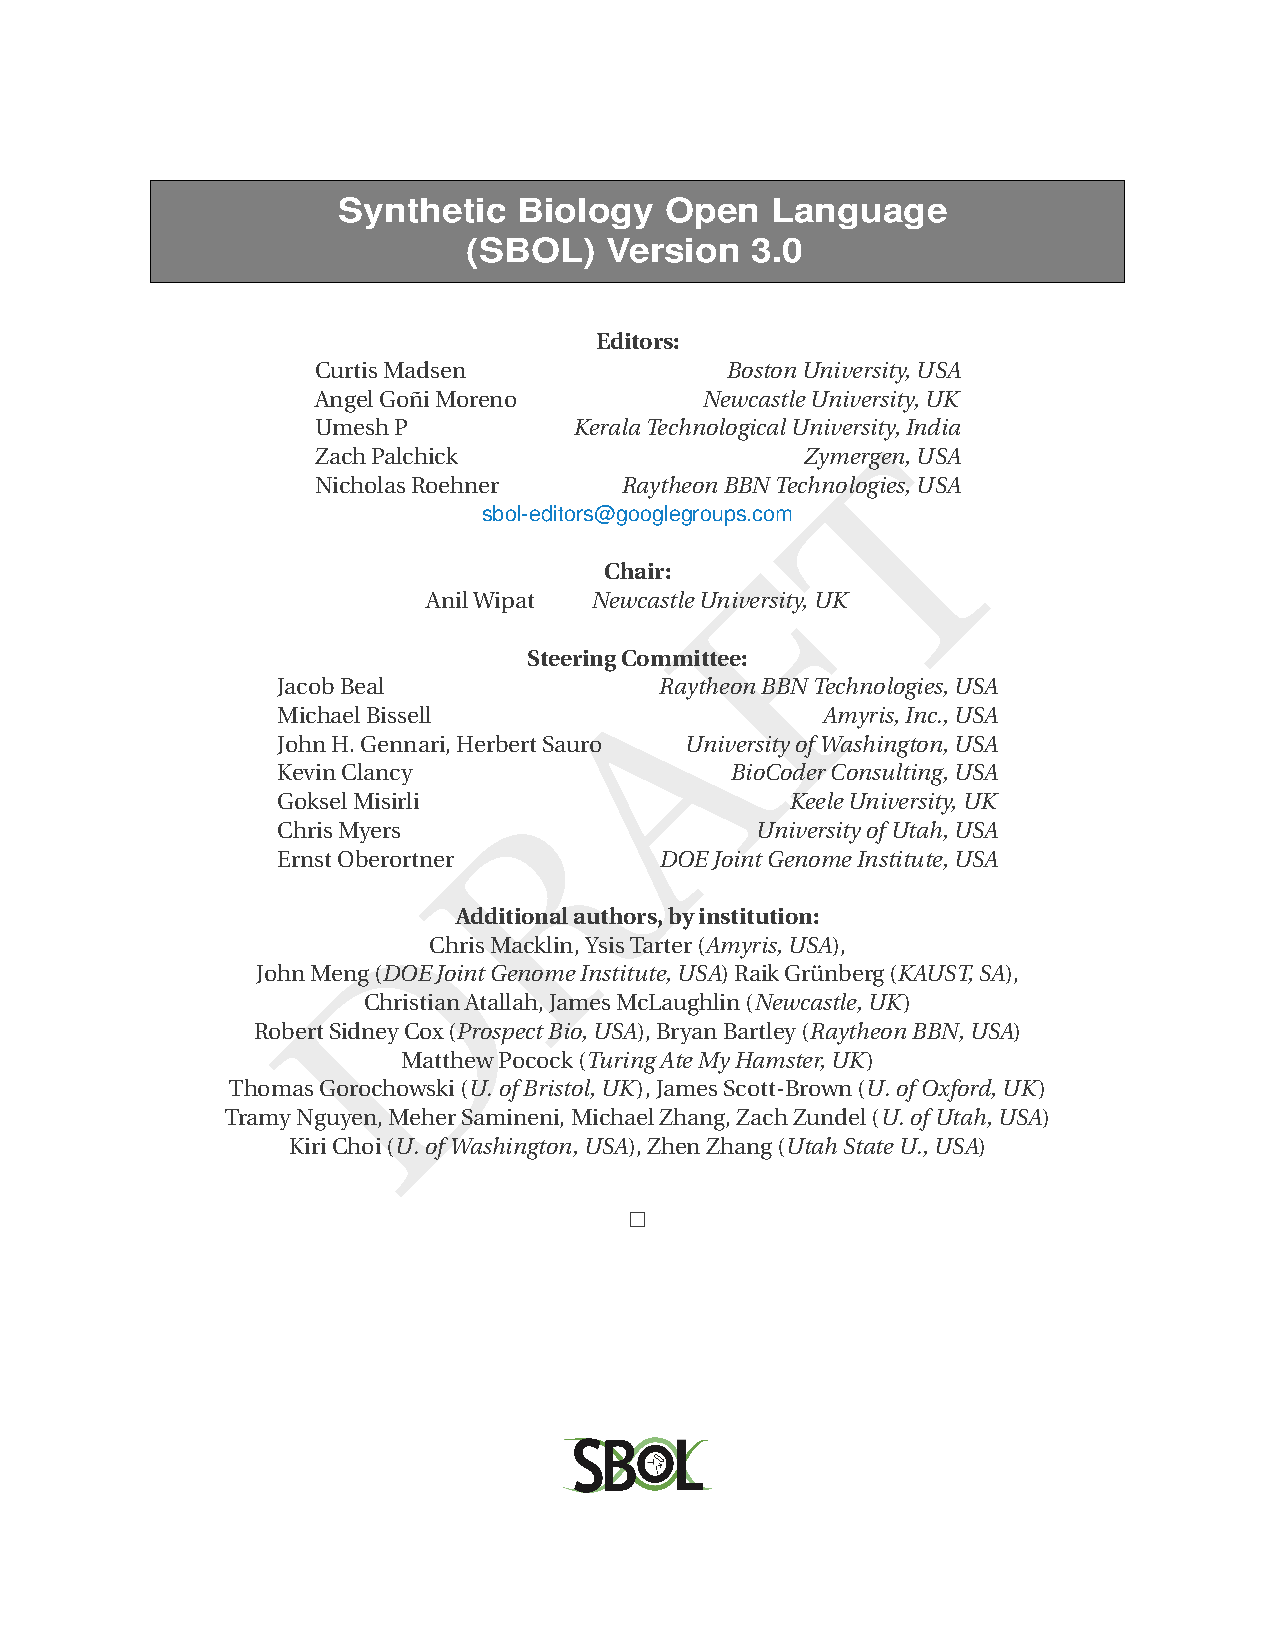
\includepdf[pages=-, offset=80 -80]{sbol3.pdf}

\end{document}